\section{Strukturen und Unionen \verweis{11}}
	\subsection{Strukturen \verweis{11.1}}
		\subsubsection{Eigenschaften}
			\begin{compactitem}
				\item Daten, welche logisch zusammengehören, können zusammengenommen werden
				\item Die Struktur ist ein zusammengesetzter Datentyp, sie setzt sich aus den Feldern zusammen
				\item Die einzelnen Felder der Strukturen können (müssen aber nicht) unterschiedliche Typen haben
				\item Jedes Feld wird mit einem innerhalb der Struktur eindeutigen Namen versehen $\rightarrow$ Strukturspezifische Präfixe für die Feldnamen (z.B. $Angestellter\_Vorname$) sind deshalb sinnlos. 
			\end{compactitem}
		
	\begin{minipage}[t]{10 cm}
		\subsubsection{Definition von Strukturtypen}
			\vspace*{-0.2cm}
			\lstinputlisting[language=C,tabsize=2]{code/strukturen1.c}
			\vspace*{0.3cm}
			\begin{compactitem}
				\item $StructName$ kann frei gewählt werden
				\item $struct$ $StructName$ ist hier ein selbst\\ definierter Typ, der weiter verwendet werden kann
				\item Der Datentyp ist definiert durch den Inhalt der\\ geschweiften Klammer
				\item Der Feldtyp kann wiederum eine Struktur sein
			\end{compactitem}
	\end{minipage}
		\hspace*{0.5cm}	
	\begin{minipage}[t]{8 cm}
		\subsubsection{Beispiel}
			\vspace*{-0.2cm}
			\lstinputlisting[language=C,tabsize=2]{code/strukturen2.c}
	\end{minipage}
	
		\subsubsection{Beispiele für die Definition von Strukturvariablen}
			\vspace*{-0.2cm}
			\lstinputlisting[language=C,tabsize=2]{code/strukturen3.c}
		\vspace*{0.3cm}		
		\subsubsection{Operationen auf Strukturvariablen}
			\begin{compactitem}
				\item Zuweisung: liegen zwei Strukturvariablen a und b vom gleichen Strukturtyp vor, so kann der Wert der einen Variablen der anderen zugewiesen werden $\rightarrow$ $a=b;$
				\item Ermittlung der Grösse der Struktur: mit $sizeof$-Operator
				\item Ermittlung der Adresse der Strukturvariablen: mit Adressoperator $\&$
			\end{compactitem}
		\subsubsection{Zugriff auf eine Strukturvariable und deren Felder}
			Der Zugriff auf ein Feld einer Strukturvariablen erfolgt über
			\begin{compactitem}
				\item den Namen der Strukturvariablen,
				\item gefolgt von einem Punkt
				\item und dem Namen des Feldes 
			\end{compactitem}			
			\vspace*{0.2cm}
			... wenn der Zugriff über einen Pointer auf eine Strukturvariable erfolgt, über
			\begin{compactitem}
				\item den Namen des Pointers,
				\item gefolgt von einem Pfeil (--\textgreater)
				\item und dem Namen des Feldes 
			\end{compactitem}
		\newpage				
		\subsubsection{Beispiele für den Zugriff auf eine Strukturvariable}
			\vspace*{-0.2cm}
			\lstinputlisting[language=C,tabsize=2]{code/strukturen4.c}
			\vspace*{0.3cm}
		\begin{minipage}[c]{8 cm}
			\subsubsection{Lage im Speicher}
				\begin{compactitem}
					\item Die Felder einer Strukturvariablen werden nacheinander gemäss der Definition in den Speicher gelegt.
					\item Gewisse Datentypen verlangen unter Umständen, dass sie auf eine Wortgrenze (gerade Adresse) gelegt werden. Dies nennt man Alignment.
					\item Durch das Alignment kann es vorkommen, dass einzelne Bytes nicht verwendet werden, d.h. im Speicher ausgelassen werden.
					\item Die Grösse einer Strukturvariablen kann nicht durch Addieren der Grössen der Felder ermittelt werden, nur $sizeof()$ liefert den genauen Wert
				\end{compactitem}
		\end{minipage}
		\hspace*{2cm}
		\begin{minipage}[c]{7 cm}
			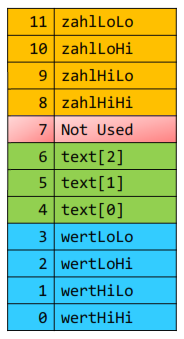
\includegraphics[width=0.5\textwidth]{pics/alignment.png}
		\end{minipage}
		\hspace*{-3cm}	
		\begin{minipage}[c]{3 cm}
			\lstinputlisting[language=C,tabsize=2]{code/strukturen5.c}
			\vspace*{0.5cm}
			Das int-Feld zahl muss auf einer geraden Adresse beginnen!
		\end{minipage}
		\subsubsection{Übergabe und Rückgabe von Strukturvariablen}
			\begin{compactitem}
				\item Strukturvariablen können komplett an Funktionen übergeben werden
				\item Der Rückgabetyp einer Funktion kann eine Struktur sein. Dabei wird die Strukturvariable direkt komplett übergeben
				\item Zu beachten ist der Kopieraufwand bei der Übergabe, bzw. Rückgabe eines Wertes. In der Praxis soll deshalb mit Pointern gearbeitet werden!
				\lstinputlisting[language=C,tabsize=2]{code/strukturen7.c} 
			\end{compactitem}
		\newpage
		\subsubsection{Initialisierung einer Strukturvariablen}
			Eine Initialisierung einer Strukturvariablen kann direkt bei der Definition der Strukturvariablen mit Hilfe einer Initialisierungsliste durchgeführt werden (Reihenfolge beachten). Natürlich muss der Datentyp $struct$ $Angestellter$ bereits bekannt sein. 
			\lstinputlisting[language=C,tabsize=2]{code/strukturen6.c} 				
	\subsection{Unions \verweis{11.2}}
		\subsubsection{Eigenschaften}
			\begin{compactitem}
				\item ähnlich wie Struktur
				\item beinhaltet auch mehrere Felder unterschiedlichen Typs
				\item im Gegensatz zur Struktur ist aber nur ein einziges Feld jeweils aktiv (abhängig vom Typ)
				\item Die Grösse einer $Union$ ist so gross wie das grösste Feld der $Union$
				\item Bei der Union sind dieselben Operationen wie bei einer Struktur definiert 
			\end{compactitem}	
		\begin{minipage}[t]{10 cm}
			\subsubsection{Definition von Uniontypen}
				\vspace*{-0.2cm}
				\lstinputlisting[language=C,tabsize=2]{code/unions1.c}
				\vspace*{0.3cm}
					\begin{compactitem}
						\item $UnionName$ kann frei gewählt werden
						\item $union$ $UnionName$ ist ein hier selbst definierter Typ, \\der weiter verwendet werden kann
						\item Der Datentyp ist definiert durch den Inhalt der \\geschweiften Klammer
						\item Der Feldtyp kann wiederum eine Union oder \\auch eine Struktur sein
					\end{compactitem}
		\end{minipage}
		\hspace*{1.5cm}	
		\begin{minipage}[t]{8 cm}
			\subsubsection{Beispiel}
				\vspace*{-0.2cm}
				\lstinputlisting[language=C,tabsize=2]{code/unions2.c}
				\vspace*{0.5cm}
				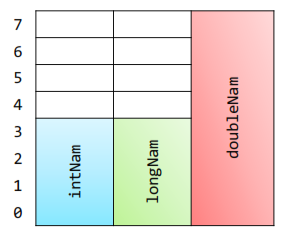
\includegraphics[width=0.5\textwidth]{pics/union.png}
		\end{minipage}
		\vspace*{0.8cm}
	\subsection{Allgemeines zu Strukturen und Unions}
		\subsubsection{Codierstil}
			\begin{compactitem}
				\item $Strukturname$ und $Unionname$ mit einem grossen Buchstaben beginnen!\\
				$struct$ $Angestellter;$\\
				$union$ $Vario;$
				\item Struktur- und Unionvariablen mit einem kleinen Buchstaben beginnen
				\item Bei Feldern von $Strukturen$ und $Union$ soll kein Präfix bei den Feldnamen verwendet werden
			\end{compactitem}
		\subsubsection{Vorsicht bei Unions}	
			\begin{compactitem}
				\item Der Programmierer muss verfolgen, welcher Typ jeweils in der $Union$ gespeichert ist. Der Datentyp, der entnommen wird, muss der sein, der zuletzt gespeichert wurde. 
			\end{compactitem}		